\documentclass[10pt]{exam}
\usepackage[phy]{template-for-exam}
\usepackage{tikz}
\usetikzlibrary{shadings,decorations.markings,arrows.meta,patterns}

\title{Bowling Ball Obstacle Course}
\author{Rohrbach}
\date{\today}

\begin{document}
\maketitle


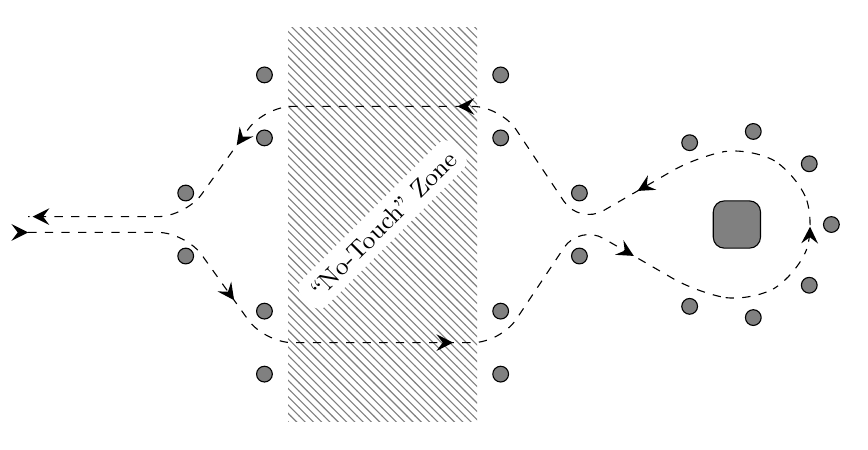
\begin{tikzpicture}[decoration={
  markings,
  mark=between positions 0 and 1 step 3cm with {\arrow[black,ultra thick]{stealth}},
   }
  ]
  \def\conerad{0.1}
  \coordinate (0) at (0,0);
  \coordinate (1) at (2,0);
  \coordinate (2) at (3,-1.5);
  \coordinate (3) at (6,-1.5);
  \coordinate (4) at (7,0);
  \coordinate (5) at (6,1.5);
  \coordinate (6) at (3,1.5);

  \foreach \c in {1,2,3,4,5,6} {
    \draw[fill=gray] (\c) +(0,0.4) circle (\conerad) +(0,-0.4) circle (\conerad);
  }


  \coordinate (turn) at (9,0);
  \draw[fill=gray] (turn) 
    +(-120:1) coordinate (a) 
    +(-120:1.2) circle (\conerad)
    %
    +(-80:1)  coordinate (b)
    +(-80:1.2) circle (\conerad)
    %
    +(-40:1)  coordinate (c)
    +(-40:1.2) circle (\conerad)
    %
    +(0:1)    coordinate (d)
    +(0:1.2) circle (\conerad)
    %
    +(40:1)   coordinate (e)
    +(40:1.2) circle (\conerad)
    %
    +(80:1)   coordinate (f)
    +(80:1.2) circle (\conerad)
    %
    +(120:1)  coordinate (g)
    +(120:1.2) circle (\conerad)
    %
    ;

  \draw[fill=gray,rounded corners] (turn) +(-0.3,0.3) rectangle +(0.3,-0.3);

  \fill[pattern=north west lines, pattern color=gray] 
    (3.3,2.5) rectangle (5.7,-2.5);
  \node[fill=white,rotate=45,rounded corners] at (4.5,0) {\small ``No-Touch'' Zone};

  \draw[
    rounded corners=10px,
    dashed,
    postaction={draw,decorate}
    ] 
    (0) ++(0,-0.1)
    -- ++(1)
    -- (2)
    -- (3)
    -- (4)
    -- (a)
    -- (b)
    -- (c)
    -- (d)
    -- (e)
    -- (f)
    -- (g)
    -- (4)
    -- (5)
    -- (6)
    -- (2,0.1)
    -- ++(-2,0);




\end{tikzpicture}

\begin{questions}


\question Why was it difficult to make the ball turn quickly? \vs
\question What direction does the ball seem to want to travel? \vs
\question What was difficult about the ``no-touch zone'' and why do you think this was? \vs 
\question Whay is it difficult to slow down the ball? \vs 
\question Would a basketball, which is similar in size but lighter in mass, have been easier or harder to move?  Explain \vs

\end{questions}

\end{document}